%2020-05-25
\documentclass[compress,xcolor=dvipsnames]{beamer}
\usepackage{tikz}
\usepackage{times}
\usepackage{calc}
\usepackage{martonsdefs}
\usepackage{graphicx}
\usepackage{marvosym}

\graphicspath{{dir1 for the UoB logo here}{dir2 for the UoB logo here}}

\useoutertheme{split}
\usecolortheme{dolphin}
\setbeamertemplate{navigation symbols}{}
\setbeamertemplate{footline}{}
\setbeamercolor{palette primary}{use=structure,bg=structure.fg!70!black,fg=white}
\setbeamercolor{subtitle}{fg=Orange}

\setbeamercolor{expl}{fg=YellowOrange}
\newcommand*{\expl}[1]{{\usebeamercolor[fg]{expl}#1}}

\setbeamercolor{gre}{fg=green!30!OliveGreen}
\newcommand*{\gre}[1]{{\usebeamercolor[fg]{gre}#1}}

\newcount\x
\newcounter{xl}
\newcounter{xr}

\title{Bertrand's paradox}
\author{M\'arton Bal\'azs}
\date{}
\institute{University of Bristol}

\begin{document}

\frame{\titlepage}
\begin{frame}{Uniform distribution}
 \animate<2-9>
 \transduration<2-4>{0.8}
 \transduration<5-7>{0.5}
 \transduration<6>{0.3}
 \transduration<7>{0.2}
 \transduration<8>{0.2}
 \transduration<9>{0.2}
 \animate<12-20>
 \transduration<12-20>{0.05}
 \animate<22-30>
 \transduration<22-30>{0.05}
 \animate<32-60>
 \transduration<32-60>{0.05}
 Pick a random point that's \emph{\expl{equally likely to be anywhere}} on \([0,\,10]\).

 \bigskip\bigskip
 \begin{center}
  \begin{tikzpicture}[x=1mm,y=1mm]
   \draw(0,0)--(50,0);
   \draw(0,1)--(0,-1)node[anchor=north]{0};
   \draw(10,-1)node[anchor=north]{2};
   \draw(20,-1)node[anchor=north]{4};
   \draw(50,1)--(50,-1)node[anchor=north]{10};
   \foreach \x in {0,5,10,...,50}\draw(\x,-1)--(\x,1);
   \draw[line width=2pt](10,0)--(20,0);
   \only<1>{
    \draw[line width=1pt](11,-1)--(13,1);
    \draw[line width=1pt](11,1)--(13,-1);
   }
   \only<2>{
    \draw[line width=1pt](40,-1)--(42,1);
    \draw[line width=1pt](40,1)--(42,-1);
   }
   \only<3>{
    \draw[line width=1pt](15,-1)--(17,1);
    \draw[line width=1pt](15,1)--(17,-1);
   }
   \only<4>{
    \draw[line width=1pt](9,-1)--(11,1);
    \draw[line width=1pt](9,1)--(11,-1);
   }
   \only<5>{
    \draw[line width=1pt](2,-1)--(4,1);
    \draw[line width=1pt](2,1)--(4,-1);
   }
   \only<6>{
    \draw[line width=1pt](41,-1)--(43,1);
    \draw[line width=1pt](41,1)--(43,-1);
   }
   \only<7>{
    \draw[line width=1pt](34,-1)--(36,1);
    \draw[line width=1pt](34,1)--(36,-1);
   }
   \only<8>{
    \draw[line width=1pt](37,-1)--(39,1);
    \draw[line width=1pt](37,1)--(39,-1);
   }
   \only<9>{
    \draw[line width=1pt](44,-1)--(46,1);
    \draw[line width=1pt](44,1)--(46,-1);
   }
   \only<10>{
    \draw[line width=1pt](15,-1)--(17,1);
    \draw[line width=1pt](15,1)--(17,-1);
   }
   \animatevalue<11-61>{\x}{0}{50}
   \only<11-20>{
    \setcounter{xl}{\the\x-1}
    \setcounter{xr}{\the\x+1}
    \draw[line width=1pt,color=red](\thexl,-1)--(\thexr,1);
    \draw[line width=1pt,color=red](\thexl,1)--(\thexr,-1);
    \draw[line width=2pt,color=red](0,0)--(\the\x,0);
   }
   \only<21-31>{
    \setcounter{xl}{\the\x-1}
    \setcounter{xr}{\the\x+1}
    \draw[line width=1pt,color=green](\thexl,-1)--(\thexr,1);
    \draw[line width=1pt,color=green](\thexl,1)--(\thexr,-1);
    \draw[line width=2pt,color=red](0,0)--(10,0);
    \draw[line width=2pt,color=green](10,0)--(\the\x,0);
   }
   \only<32->{
    \setcounter{xl}{\the\x-1}
    \setcounter{xr}{\the\x+1}
    \draw[line width=1pt,color=red](\thexl,-1)--(\thexr,1);
    \draw[line width=1pt,color=red](\thexl,1)--(\thexr,-1);
    \draw[line width=2pt,color=red](0,0)--(10,0);
    \draw[line width=2pt,color=green](10,0)--(20,0);
    \draw[line width=2pt,color=red](20,0)--(\the\x,0);
   }
  \end{tikzpicture}
 \end{center}
 \[
  \Pb\{
   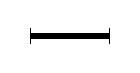
\begin{tikzpicture}[x=1mm,y=1mm]
    \draw[line width=2pt](0,0)--(10,0);
    \draw(0,-1)--(0,1);
    \draw(10,-1)--(10,1);
   \end{tikzpicture}
  \}=\alt<62>{
   %\makebox[6cm][l]{$
   \parbox[c][2cm][c]{4.1cm}{$
    \frac{
     |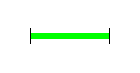
\begin{tikzpicture}[x=1mm,y=1mm]
      \draw[line width=2pt,color=green](0,0)--(10,0);
      \draw(0,-1)--(0,1);
      \draw(10,-1)--(10,1);
     \end{tikzpicture}|
    }
    {%
     |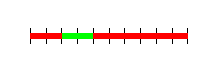
\begin{tikzpicture}[x=0.4mm,y=0.4mm]
      \foreach \x in {0,5,10,...,50}\draw(\x,-2.5)--(\x,2.5);
      \draw(0,0)--(50,0);
      \draw[line width=2pt,color=red](0,0)--(10,0);
      \draw[line width=2pt,color=green](10,0)--(20,0);
      \draw[line width=2pt,color=red](20,0)--(50,0);
     \end{tikzpicture}|
    }=\frac2{10}=\frac15.
   $}
  }
  {
   %\makebox[6cm][l]{?}
   \parbox[c][2cm][c]{4.1cm}{?}
  }
 \]
\end{frame}
\begin{frame}{Random chords and a question}
 \animate<4-7>
 \transduration<4-7>{1.2}
 \animate<13-16>
 \transduration<13-16>{2.5}
 \begin{center}
  \begin{tikzpicture}[x=0.25mm,y=0.25mm]
   \draw(0,0)circle(100);
   \fill(0,0)circle(1);
   \only<1>{
    \draw(0,0)--(87,50)node[midway,above,style=sloped]{\(1\)};
   }
   %Wow TikZ can draw directly in polar coordinates!
   \only<2>{
    \draw[thick](23:100)--(161:100);
   }
   \only<3>{
    \draw[thick](31:100)--(32:100);
   }
   \only<4>{
    \draw[thick](262:100)--(136:100);
   }
   \only<5>{
    \draw[thick](234:100)--(135:100);
   }
   \only<6>{
    \draw[thick](59:100)--(200:100);
   }
   \only<7>{
    \draw[thick](170:100)--(184:100);
   }
   \only<8>{
    \draw[thick](215:100)--(269:100);
   }
   \only<9-10>{
    \draw[thick,color=blue](30:100)--(150:100)--(270:100)--(30:100);
   }
   \only<11>{
    \draw[thick,color=green](23:100)--(161:100);
    \draw[thick,color=blue](152:100)--(272:100)--(32:100)--(152:100);
   }
   \only<12>{
    \draw[thick,color=red](31:100)--(32:100);
    \draw[thick,color=blue](91.5:100)--(211.5:100)--(331.5:100)--(91.5:100);
   }
   \only<13>{
    \draw[thick,color=green](262:100)--(136:100);
    \draw[thick,color=blue](259:100)--(19:100)--(139:100)--(259:100);
   }
   \only<14>{
    \draw[thick,color=red](234:100)--(135:100);
    \draw[thick,color=blue](244.5:100)--(4.5:100)--(124.5:100)--(244.5:100);
   }
   \only<15>{
    \draw[thick,color=green](59:100)--(200:100);
    \draw[thick,color=blue](189.5:100)--(309.5:100)--(69.5:100)--(189.5:100);
   }
   \only<16>{
    \draw[thick,color=red](170:100)--(184:100);
    \draw[thick,color=blue](237:100)--(357:100)--(117:100)--(237:100);
   }
   \only<17>{
    \draw[thick,color=red](215:100)--(269:100);
    \draw[thick,color=blue](302:100)--(62:100)--(182:100)--(302:100);
   }
  \end{tikzpicture}
  \uncover<2->{
   \[
    \uncover<10->{
     \Pb\{
    }
    \text{\emph{random chord}}
    \uncover<10->{
     \text{ is longer than one side of the }
    }
    \uncover<9->{
     
\begin{tikzpicture}[x=1.8mm,y=1.8mm]
      \draw[color=blue](30:1)--(150:1)--(270:1)--(30:1);
     \end{tikzpicture}
    }
    \uncover<10->{
     \} \text{?}
    }
   \]
  }
 \end{center}
\end{frame}
\begin{frame}{Answer: \(\tfrac12\)}
 \animate<3-26>
 \transduration<3-26>{0.1}
 \animate<28-51>
 \transduration<28-51>{0.1}
 \begin{center}
  \begin{tikzpicture}[x=0.25mm,y=0.25mm]
   \draw(0,0)circle(100);
   \fill(0,0)circle(1);
   \draw[thick,color=blue](30:100)--(150:100)--(270:100)--(30:100);
   \draw(0,0)--(0,50)node[midway,left]{\(\tfrac12\)};
   \only<1>{
    \draw(0,0)--(87,50)node[midway,above,style=sloped]{\(1\)};
   }
   \only<2->{
    \draw(0,50)--(0,100)node[midway,left]{\(\tfrac12\)};
   }
   \animatevalue<2-52>{\x}{0}{100}
   \only<2-27>{
    \draw[thick,color=green](-100,\the\x)--(100,\the\x);
    \draw[line width=2pt,color=green](0,0)--(0,\the\x);
   }
   \only<28-52>{
    \draw[thick,color=red](-100,\the\x)--(100,\the\x);
    \draw[line width=2pt,color=green](0,0)--(0,50);
    \draw[line width=2pt,color=red](0,50)--(0,\the\x);
   }
   \fill[white,even odd rule](0,0)circle[radius=100.2]circle[radius=141.8];
  \end{tikzpicture}
 \end{center}
 \uncover<2->{
  Distance from center:
 }
 \uncover<52>{
  \(\frac{\gre{\frac12}}{\gre{\frac12}+\alert{\frac12}}=\frac12.\)
 }
\end{frame}
\begin{frame}{Wait\dots it's \(\tfrac13\)!}
 \animate<3-21>
 \transduration<3-21>{0.1}
 \animate<23-41>
 \transduration<23-41>{0.1}
 \animate<43-61>
 \transduration<43-61>{0.1}
 \begin{center}
  \begin{tikzpicture}[x=0.25mm,y=0.25mm]
   \draw(0,0)circle(100);
   \fill(0,0)circle(1);
   \draw[thick,color=blue](30:100)--(150:100)--(270:100)--(30:100);
   \draw(30:100)--++(120:60);
   \draw(30:100)--++(300:60);
   \draw(30:100)+(120:20)arc(120:300:20)node[pos=0.1,left]{\small{\(60^\text o\)}}node[pos=0.63,left]{\small{\(60^\text o\)}}node[pos=0.8,below]{\small{\(60^\text o\)}};
   \animatevalue<2-62>{\x}{30}{390}
   \setcounter{xl}{\the\x/2+105}
   \only<2-21>{
    \draw[thick,color=red](30:100)--(\the\x:100);
    \draw[line width=2pt,color=red](30:100)+(120:20)arc(120:\thexl:20);
   }
   \only<22-42>{
    \draw[thick,color=green](30:100)--(\the\x:100);
    \draw[line width=2pt,color=red](30:100)+(120:20)arc(120:180:20);
    \draw[line width=2pt,color=green](30:100)+(180:20)arc(180:\thexl:20);
   }
   \only<43-62>{
    \draw[thick,color=red](30:100)--(\the\x:100);
    \draw[line width=2pt,color=red](30:100)+(120:20)arc(120:180:20);
    \draw[line width=2pt,color=green](30:100)+(180:20)arc(180:240:20);
    \draw[line width=2pt,color=red](30:100)+(240:20)arc(240:\thexl:20);
   }
   \fill[white,even odd rule](0,0)circle[radius=141]circle[radius=141.8];
  \end{tikzpicture}
 \end{center}
 \uncover<2->{
  Angle:
 }
 \uncover<62>{
  \(\frac{\gre{60^\text o}}{\alert{60^\text o}+\gre{60^\text o}+\alert{60^\text o}}=\frac13.\)
 }
\end{frame}
\begin{frame}{Oh wait\dots it's \(\tfrac14\)!}
 \animate<12-35>
 \transduration<12-35>{0.1}
 \animate<37-60>
 \transduration<37-60>{0.1}
 \begin{center}
  \begin{tikzpicture}[x=0.25mm,y=0.25mm]
   \only<1>{
    \draw(0,0)--(87,50)node[midway,above,style=sloped]{\(1\)};
   }
   \only<2-4>{%37, 39
    \draw[line width=1pt](34,36)--(40,42);
    \draw[line width=1pt](34,42)--(40,36);
   }
   \only<3>{
    \draw[thick](37,39)--++(136.5:90);
    \draw[thick](37,39)--++(316.5:90);
    \draw(0,0)--(37,39);
   }
   \only<4>{
    \draw[thick,color=red](37,39)--++(136.5:90);
    \draw[thick,color=red](37,39)--++(316.5:90);
    \draw(0,0)--(37,39);
    \draw[thick,color=blue](346.5:100)--(106.5:100)--(226.5:100)--(346.5:100);
   }
   \only<5-7>{%9, 26
    \draw[line width=1pt](6,23)--(12,29);
    \draw[line width=1pt](6,29)--(12,23);
   }
   \only<6>{
    \draw[thick](9,26)--++(160.9:100);
    \draw[thick](9,26)--++(340.9:100);
    \draw(0,0)--(9,26);
   }
   \only<7>{
    \draw[thick,color=green](9,26)--++(160.9:100);
    \draw[thick,color=green](9,26)--++(340.9:100);
    \draw(0,0)--(9,26);
    \draw[thick,color=blue](10.9:100)--(130.9:100)--(250.9:100)--(10.9:100);
   }
   \only<8-10>{%53, -26
    \draw[line width=1pt](50,-29)--(56,-23);
    \draw[line width=1pt](50,-23)--(56,-29);
   }
   \only<9>{
    \draw[thick](53,-26)--++(63.9:100);
    \draw[thick](53,-26)--++(243.9:100);
    \draw(0,0)--(53,-26);
   }
   \only<10>{
    \draw[thick,color=red](53,-26)--++(63.9:100);
    \draw[thick,color=red](53,-26)--++(243.9:100);
    \draw(0,0)--(53,-26);
    \draw[thick,color=blue](273.9:100)--(33.9:100)--(153.9:100)--(273.9:100);
   }
   \animatevalue<11-61>{\x}{0}{100}
   \only<11-36>{
    \draw[thick,color=green](-100,\the\x)--(100,\the\x);
    \fill[color=green](0,0)circle(\the\x);
   }
   \only<37-61>{
    \draw[thick,color=red](-100,\the\x)--(100,\the\x);
    \fill[color=green](0,0)circle(50);
    \fill[red,even odd rule](0,0)circle[radius=50]circle[radius=\the\x];
   }
   \fill(0,0)circle(1);
   \only<1-3,5-6,8-9,11->{
    \draw[thick,color=blue](30:100)--(150:100)--(270:100)--(30:100);
   }
   \only<11->{
    \setcounter{xl}{\the\x-3}
    \setcounter{xr}{\the\x+3}
    \draw[line width=1pt](-3,\thexl)--(3,\thexr);
    \draw[line width=1pt](-3,\thexr)--(3,\thexl);
   }
   \draw(0,0)circle(100);
   \only<1,11->{
    \draw(0,0)--(0,50)node[midway,left]{\(\tfrac12\)};
   }
   \fill[white,even odd rule](0,0)circle[radius=100.2]circle[radius=141.8];
  \end{tikzpicture}
 \end{center}
 \uncover<2->{
  Midpoint:
 }
 \uncover<61>{
  \(\frac{|
   \raisebox{-1.5pt}{
    \begin{tikzpicture}[x=0.7mm,y=0.7mm]
     \fill[color=green](0,0)circle(1);
     \fill[white,even odd rule](0,0)circle[radius=1]circle[radius=2];
    \end{tikzpicture}
   }
  |}{|
   \raisebox{-1.5pt}{
    
\begin{tikzpicture}[x=0.7mm,y=0.7mm]
     \fill[color=green](0,0)circle(1);
     \fill[red,even odd rule](0,0)circle[radius=1]circle[radius=2];
    \end{tikzpicture}
   }
  |}=\frac{\gre{\bigl(\frac12\bigr)^2\cdot\pi}}{1^2\cdot\pi}=\frac14.\)
 }
\end{frame}
\begin{frame}{Answer: \(\tfrac12\)? \(\tfrac13\)? \(\tfrac14\)? }
 \structure{\emph{Come to Bristol and we'll show you how to properly define a probability space!} \Smiley{}}

 \vskip2cm
 \begin{center}
  \includegraphics[height=1.5cm]{logo.eps}
 \end{center}
\end{frame}
\end{document}
